\XeTeXgenerateactualtext=1
\ifdefined\HANDOUT
  \documentclass[fontset=adobe, t, handout]{ctexbeamer}
\else
  \documentclass[fontset = adobe, t]{ctexbeamer}
\fi

% 载入需要的宏包
% 加载宏包
%===================注意======================%
% 在调用beamer.cls宏包后,以下宏包将自动调用,
% 不应单独调用这些宏包,以免发生冲突
% amsfonts, amsmath, amssymb, amsthm, 
% enumerate, geometry, graphics, graphicx, 
% hyperref, url, 
% ifpdf, keyval, xcolor, xxcolor
% =============================================%
% TiKZ绘图宏包
\usepackage{tikz}

% 绘制内存结构图
\usepackage{bytefield}

% 编排代码
\usepackage{minted}

% 绘制UML图
\usepackage{pgf-umlcd}

%%% Local Variables: 
%%% mode: latex
%%% TeX-master: "../main.tex"
%%% End:


% 进行必要的设置
% ====================================================================================
% bytefield绘图设置
% 调整表格的垂直对齐方式
\newcommand{\descbox}[1]{\parbox[c][0.7\baselineskip]{0.95\width}{%
\raggedright #1\vfill}}
% 用于绘制无标记内存图中一个内存块的命令,其开始地址在底部,结束地址在顶部(基于bytefield宏包)
% 语法:
% \memsec{结束地址}{开始地址}{以行为单位的高度}{盒子中的文字}
\newcommand*\istempaddr[1]{\IfStrEq{}{#1}{}{0X#1}}
\newcommand{\memsec}[4]{%
  % 定义memsection的高度
  %
  %\tiny
  \bytefieldsetup{bitheight=#3\baselineskip}%
  \bitbox[]{5}{%    
    \tiny \texttt{\istempaddr{#1}}%0X#1}% 结束地址
    \\
    % 留出空白
    \vspace{#3\baselineskip}
    \vspace{-1.6\baselineskip}
    \vspace{-#3pt}
    \tiny \texttt{\istempaddr{#2}}%0X#2}% 开始地址
  }%
  \bitbox{4}{\tiny \texttt{#4}}% 盒子里的内容 %\vspace{-0.9\baselineskip}
}

% 定义绘制有标记内存的命令(基于bytefield宏包)
% 创建计算机内存映像的自定义命令,
% 起始地址位于低部,结束地址位于顶部
% 语法:
% \memsection[标记符号]{结束地址}{起始地址}{内存单元高度}{内存单元中的内容}
% 其中标记符号为可选项,可以是任何符合LaTeX语法的内容
\newcommand{\memseclab}[5][]{
  %\tiny
  \bytefieldsetup{bitheight=#4\baselineskip} % 内存单元的高度
  \bitbox[]{10}{%标记符号及地址盒子,参数为总宽度
    \raggedleft%右对齐
    \texttt{\tiny\istempaddr{#2}}% 结束地址
    \\%换行
    % 设置结束地址与起始地址之间的空白
    \vspace{#4\baselineskip}
    \vspace{-1.5\baselineskip}
    \vspace{-#4pt} % 
    {\tiny\texttt{#1}}%\hspace{1em}
    \texttt{\tiny\istempaddr{#3}}% 起始地址
  }~
  \bitbox{4}{\tiny \texttt{#5}} % 内存单元盒子
}

% 自定义垂直省略号
\makeatletter
\DeclareRobustCommand{\rvdots}{%
  \vbox{
    \baselineskip3\p@\lineskiplimit\z@
    \kern-\p@
    \hbox{.}\hbox{.}\hbox{.}
  }}
\makeatother
% ====================================================================================

% ====================================================================================
% 重定义强调字体的代码,解决默认强调字体是italic,此时中文会用楷体代替,
% 在此设置为加粗,注意需要使用etoolbox宏包
\makeatletter
\let\origemph\emph
\newcommand*\emphfont{\normalfont\bfseries}
\DeclareTextFontCommand\@textemph{\emphfont}
\newcommand\textem[1]{%
  \ifdefstrequal{\f@series}{\bfdefault}
    {\@textemph{\CTEXunderline{#1}}}
    {\@textemph{#1}}%
}
\RenewDocumentCommand\emph{s o m}{%
  \IfBooleanTF{#1}
    {\textem{#3}}
    {\IfNoValueTF{#2}
      {\textem{#3}\index{#3}}
      {\textem{#3}\index{#2}}%
     }%
}
\makeatother   
% ====================================================================================

% 代码显示模式设置(基于minted宏包)
% ====================================================================================
\usemintedstyle{default}  %codeblocks模式

% 定义排版C语言代码命令
\setminted{fontsize=\tiny, breaklines=true,
  breakautoindent=false}
\newmintinline{c}{fontsize=\normalsize, autogobble}
\newmintinline[cinlinett]{c}{fontsize=\normalsize, escapeinside=||, autogobble}
\newmintinline[cinttscr]{c}{fontsize=\scriptsize, escapeinside=||, autogobble}
\newmintinline[cinttfts]{c}{fontsize=\footnotesize, escapeinside=||, autogobble}
\newmintinline[cintttny]{c}{fontsize=\tiny, escapeinside=||, autogobble}
\newmintinline[cinttlrg]{c}{fontsize=\large, escapeinside=||, autogobble}
\newminted{c}{frame=lines, autogobble}
\newminted[ctt]{c}{mathescape,frame=lines,escapeinside=||, autogobble}
\newmintedfile{c}{frame=lines}%linenos=true,
\newmintedfile[cfilett]{c}{frame=lines,escapeinside=||}%linenos=true,
\newmintedfile[cfttscr]{c}{fontsize = \scriptsize, frame=lines,escapeinside=||}%linenos=true,
\newmintedfile[cfiletikz]{c}{frame=lines}%linenos=true,
% ====================================================================================

% TikZ宏包扩展
% ====================================================================================
\usetikzlibrary{graphs}
\usetikzlibrary{mindmap,trees}
\tikzset{every concept/.style={minimum size=1cm, text width=1.5cm}}
\usetikzlibrary{shapes,arrows,chains}
\usetikzlibrary{positioning}
\usetikzlibrary{calc}
\usetikzlibrary{arrows.meta}
\usetikzlibrary{decorations.pathreplacing}
\usetikzlibrary{tikzmark}
\usetikzlibrary{shapes.geometric}
\usetikzlibrary{decorations.text}
\usetikzlibrary{matrix}
\usetikzlibrary{backgrounds}

% 流程图属性设置
% ====================================================================================
% 各参数默认值
\flowchartset{
  free color = green, % 自由连线颜色(默认取green)
  norm color = blue, % 常规连线颜色(默认取blue)
  cong color = red, % 关联连线颜色(默认取red)
  proc fill color = orange!10, % 顺序处理框填充颜色(默认取白色)
  test fill color = green!30, % 判断框填充颜色(默认取白色)
  io fill color = blue!30, % 输入/输出框填充颜色(默认取白色)
  term fill color = red!30, % 开始/结束框填充颜色(默认取白色)
  flow line width = 1.3\pgflinewidth, % 各类流程线线条宽度(默认取当前线条宽度)
}
% ====================================================================================

% 设置动画显示样式
% ====================================================================================
\tikzset{
  invisible/.style={opacity=0},
  visible on/.style={alt={#1{}{invisible}}},
  alt/.code args={<#1>#2#3}{%
    \alt<#1>{\pgfkeysalso{#2}}{\pgfkeysalso{#3}} % \pgfkeysalso doesn't change the path
  },
}
% ====================================================================================

%%%%%%%%%% 绘制链表数据结构需要的命令TiKz%%%%%%%%
% ====================================================================================
\usetikzlibrary{shapes,arrows,calc}
\newcommand{\data}{data \nodepart{second} \phantom{null}}

\tikzstyle{ptr}  = [draw, -latex', blue]
\tikzstyle{head} = [rectangle, draw, text height=3mm, text width=3mm, text centered, node distance=3cm, inner sep=0pt]
\tikzstyle{data} = [rectangle split, rectangle split parts=2, draw, text centered, minimum height=3em]
% ====================================================================================

% 改变脚注的符号
% ====================================================================================
\setbeamerfont{footnote}{size=\zihao{7}} % 改变脚注字号
\makeatletter
\def\@fnsymbol#1{\ensuremath{\ifcase#1\or *\or \dagger\or \ddagger\or
   \mathsection\or \mathparagraph\or \|\or **\or \dagger\dagger
   \or \ddagger\ddagger \else\@ctrerr\fi}}
\makeatother
\renewcommand{\thefootnote}{\fnsymbol{footnote}}
% ====================================================================================

% 定义C语言中的专有名词命令
% ====================================================================================
\newcommand{\cb}{\texttt{Code::Blocks}}
\newcommand{\mww}{\texttt{MinGW-w64}}
\newcommand{\mfile}{\qtmark{\texttt{Makefile}}}
\newcommand{\vs}{\texttt{Visual Studio}}
\newcommand{\gcc}{\texttt{gcc}}
\newcommand{\db}{\texttt{DEBUG}}
\newcommand{\dbger}{\texttt{Debugger}}
\newcommand{\gdb}{\texttt{gdb}调试器}
\newcommand{\cdb}{\texttt{cdb}调试器}
\newcommand{\gdbcmd}{\texttt{(gdb)}}
\newcommand{\scf}{\cinline[fontsize = \scriptsize]{scanf()}}
\newcommand{\ptf}{\cinline{printf()}}
\newcommand{\rn}{\cinline{'\n'}}
\newcommand{\cch}[1]{\cinline{'#1'}}
\newcommand{\lumos}{Linux、Unix、Mac OS}
\newcommand{\win}{Windows}
\newcommand{\unix}{UNIX}
\newcommand{\lnx}{Linux}

\newcommand{\cl}{{C语言}}
\newcommand{\nint}{{\cinline{int}}}
\newcommand{\flt}{{\cinline{float}}}
\newcommand{\snint}{{\cinline{short int}}}
\newcommand{\lint}{{\cinline{long int}}}
\newcommand{\llint}{{\cinline{long long int}}}
\newcommand{\ldb}{{\cinline{long double}}}
\newcommand{\sch}{{\cinline{signed char}}}
\newcommand{\sint}{{\cinline{signed int}}}
\newcommand{\ssint}{{\cinline{signed short int}}}
\newcommand{\slint}{{\cinline{signed long int}}}
\newcommand{\sllint}{{\cinline{signed long long int}}}
\newcommand{\usch}{{\cinline{unsigned char}}}
\newcommand{\usint}{{\cinline{unsigned int}}}
\newcommand{\ussint}{{\cinline{unsigned short int}}}
\newcommand{\uslint}{{\cinline{unsigned long int}}}
\newcommand{\usllint}{{\cinline{unsigned long long int}}}

% 路径设置
% ====================================================================================
\graphicspath{{figure/}}%图片所在的目录
% ====================================================================================


%%% Local Variables: 
%%% mode: latex
%%% TeX-master: "../main.tex"
%%% End: 


% Information
\title[学位论文\\ \nwafuthesis{}模板简介]{西北农林科技大学学位论文\\ \nwafuthesis{}模板简介}
\subtitle{A Short Introduction of \nwafuthesis}
\author[Nine, G.]{耿楠}
\institute[教发中心]{西北农林科技大学\quad 教学发展中心}
\date{\tosemester}
\titlegraphic{%
  \vspace{3.4cm}
  \qrcode[hyperlink, height=1.6cm]{https://github.com/registor/shortintronwafuthesis/}}

\begin{document}

\maketitle

\section[\LaTeX 简介]{\LaTeX 简介}
\subsection[为什么?]{为什么要用\LaTeX{}}
\begin{frame}{为什么要用\LaTeX?}{学位论文排版的需求}
  \begin{spacing}{0.85}
  \begin{itemize}% \setlength\itemsep{1em}
  \item 标准、规范\alert{严格}
    \begin{itemize}
    \item \alert{国家}标准
      \begin{itemize}
      \item 《学位论文编写规则》(GB/T7713.1-2006)
      \item 《国际单位制及其应用》(GB3100-1993)
      \item 《有关量、单位和符号的一般原则》(GB3101-1993)
      \item 《信息与文献参考文献著录规则》(GB/T7714-2015)
      \item $\ldots$
      \end{itemize}
    \item \alert{学校}规定和规范
      \begin{itemize}
      \item \href{https://yjshy.nwafu.edu.cn/xwgl/xwlwxzgf/index.htm}{研究生学位论文\alert{写作指南}}
      \item \href{https://yjshy.nwafu.edu.cn/xwgl/xwlwxzgf/127000.htm}{研究生学位论文\enquote{参考文献}\alert{著录规则}}
      \item \href{https://jiaowu.nwsuaf.edu.cn/tzgg/34321.htm}{本科生学位论文(设计)\alert{写作规范}}      
      \end{itemize}
    \end{itemize}
  \item 篇幅\alert{长}
    \begin{itemize}
    \item 本科:约15000字+约5000字符译文,30$\sim$50页(A4)
    \item 硕士:约30000$\sim$50000字,50$\sim$80页(A4)
    \item 博士:字数100000+,100$\sim$150页(A4)
    \end{itemize}  
  \item 修改、修订\alert{频繁}
    \begin{itemize}
    \item 增、删、改(公式、图表、参考文献)
    \item 交叉引用
    \item \alert{自动化}
    \end{itemize}  
  % \item 高效、便捷
  %   \begin{itemize}
  %   \item \href{https://github.com/registor/nwafuthesis}{\nwafuthesis 模板}
  %   \end{itemize}
  \end{itemize}
  \end{spacing}
\end{frame}

\begin{frame}{为什么要用\LaTeX?}{自由的召唤}
  \begin{columns}[c]
    \column{0.05\textwidth}
    \column{0.4\textwidth}
    \begin{itemize} \setlength\itemsep{1em}
    \item \alert{懒人}的梦想
    \item 对\alert{美}的追求
    \item \alert{自由}的召唤
    \item \alert{正版}的限制
    \item 平台的\alert{稳定}
    \item \alert{开源}的系统
    \item \alert{倒版倒平台}
    \item \alert{导师}的要求
    \item \alert{投稿}的需求
    \item $\ldots$\hphantom{倒版倒a}%为了对齐,设置一个占位空间
    \end{itemize}
    \column{0.5\textwidth}
    \begin{center}
      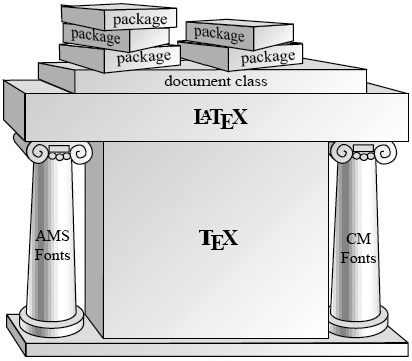
\includegraphics[width=0.45\textwidth]{latexframe}\\
      
\includegraphics[width=0.3\textwidth]{titlepage}\\%scale=0.05
      贴心\alert{秘书}
    \end{center}
  \end{columns}
\end{frame}

\begin{frame}{为什么要用\LaTeX?}{Office的那点事}%
  \centering
  
\includegraphics[height=.65\textheight]{msoffice2013.png}\\[.5em]
  \msoffice{} \footnote[frame,1]{及其类似软件(LibreOffice, etc.)}%为了在
                                %beamer中显示脚注,需要使用参数[frame]
  功能异常强大\ldots
\end{frame}

% \begin{frame}{为什么要用\LaTeX?}{与Word比较}
%   \begin{itemize}
%   \item 使用难度
%   \end{itemize}
%   \centering
%   \vspace{2ex}
%   \begin{tikzpicture}[scale=0.9, every node/.style={scale=0.9}]
%     \pgfplotsset{every axis/.append style={line width=1pt}}
%     \begin{axis}[%
%       axis x line=bottom,
%       axis y line=left,
%       ymin=0,
%       xtick={},
%       xticklabels={},
%       xlabel near ticks,
%       ytick={},
%       yticklabels={},
%       ylabel near ticks,
%       xlabel={文档大小和复杂性\footnote[frame]{\href{http://www.pinteric.com/miktex.html}{Marko
%       Pinteric: http://www.pinteric.com/miktex.html}}},
%       ylabel={耗时和难度},
%       ]
%       \begin{scope}[decoration={random steps,segment length=1pt,amplitude=0.1pt},decorate]
%         \addplot [msofficecolour, samples=130, domain=0:2] {1+2*x^3}
%                   node[near end, sloped, above] {\msoffice}
%                   node[anchor=east, pos=.98] {\tiny (我不玩了!再见\ldots)};
%          \addplot [latexcolour, samples=130, domain=0:2] {2+x}
%                   node[near end, sloped, above] {\latex};
%       \end{scope}
%     \end{axis}
%   \end{tikzpicture}
% \end{frame}

% \begin{frame}{为什么要用\LaTeX?}{与Word比较}
%   \begin{itemize}
%   \item 学习曲线
%   \end{itemize}
%   \centering
%   \vspace{2ex}
%   \begin{tikzpicture}[scale=0.9, every node/.style={scale=0.9}]
%     \pgfplotsset{every axis/.append style={line width=1pt}}
%     \begin{axis}[%
%       axis x line=bottom,
%       axis y line=left,      
%       xtick={},
%       xticklabels={},
%       xlabel near ticks,
%       ytick={},
%       yticklabels={},
%       ylabel near ticks,
%       xlabel={需求复杂度/经验},
%       ylabel={学习难度},
%       xmin=0,
%       xmax=4,
%       ymin=0,
%       ymax=4,
%       ]
%       % 用贝塞尔曲线(Bézier curve)绘制学习曲线示意图
%       \begin{scope}[decoration={random steps,segment length=1pt,amplitude=0.1pt},decorate]
%         \draw[color=msofficecolour] (0,0) .. controls (3.8,0.00) and (1.5,3.8)
%         .. (3.8,3.8) node[near end, sloped, above] {\msoffice};
%         \draw[latexcolour] (0,0) .. controls (0.1,1.8) and (1.8,1.8)
%         .. (3.8,1.6) node[xshift = -0.8cm, sloped, above] {\latex};
%       \end{scope}
%     \end{axis}
%   \end{tikzpicture}
% \end{frame}

% \begin{frame}{为什么要用\LaTeX?}{Word的那点事}
%   \stretchon
%   \begin{itemize}
%   \item \msoffice 是 \wysiwyg
%     \begin{itemize}
%     \item ``\textsc{What You See Is What You \emph{Get}}''
%     \item 格式和结构有时是含蓄的
%     \item 貌似易用,但对排版只能进行有限的控制
%     \end{itemize}
%     %\myrule
%   \item \latex 是 \wysiwym
%     \begin{itemize}
%     \item ``\textsc{What You See Is What You \emph{Mean}}''
%     \item 格式与结构清晰
%     \item 貌似繁琐,实则是对版面可以进行详细的控制
%     \end{itemize}
%   \end{itemize}
%   \stretchoff
% \end{frame}

% \begin{frame}{为什么要用\LaTeX?}{Word的那点事}
%   \stretchon
%   \begin{itemize}
%   \item 玻璃瓶和塑料瓶
%     \begin{itemize}
%     \item \msoffice 是玻璃瓶$\Rightarrow$ \alert{易碎}
%     \item \latex 是塑料瓶$\Rightarrow$ \alert{皮实}
%     \end{itemize}
%   \item 模板
%     \begin{itemize}
%     \item \msoffice 往往是\alert{规定}$\Rightarrow$ 沦落为低级趣味的\alert{格式刷}
%     \item \latex 强制使用模板$\Rightarrow$ 真正实现了\alert{内容与格式的分离}
%     \end{itemize}
%   \item 轮子的故事
%     \begin{itemize}
%     \item \msoffice$\Rightarrow$ \alert{ 发明和制造}轮子
%     \item \latex$\Rightarrow$  \alert{ 使用}轮子
%     \end{itemize}
%   \item 两条腿走路
%     \begin{itemize}      
%     \item 不会用
%       \begin{itemize}
%       \item \msoffice $\Rightarrow$ 文档难看,格式丑
%       \item \latex $\Rightarrow$ 无法编译,\alert{没有文档}
%       \end{itemize}
%     \item 会用
%       \begin{itemize}
%       \item \msoffice $\Rightarrow$ \alert{难看}的文档
%       \item \latex $\Rightarrow$ 漂亮的文档
%       \end{itemize}
%     \item 用的好
%       \begin{itemize}
%       \item \msoffice $\Rightarrow$ \alert{完美}的文档
%       \item \latex $\Rightarrow$ \alert{完美}的文档
%       \end{itemize}
%     \end{itemize}    
%   \end{itemize}
%   \stretchoff
% \end{frame}

%%% Local Variables:
%%% mode: latex
%%% TeX-master: "../main.tex"
%%% End:


% \subsection[是什么?]{什么是\LaTeX{}}
% \section[安装\LaTeX{}]{安装\LaTeX{}}
% \subsection[下载软件]{下载软件}
% \subsection[注意事项]{注意事项}
% \section[学习\LaTeX{}]{学习\LaTeX{}}
% \subsection[命令行]{命令行操作}
% \subsection[学习资源]{学习资源}
% \subsection[文档结构]{文档结构}
% \subsection[错误处理]{错误处理}
% \section[\nwafuthesis{}模板]{\nwafuthesis{}模板}
% \subsection[开发需求]{开发需求}
% \subsection[模板下载]{模板下载}
% \subsection[模板使用]{模板使用}
% \subsection[TeXstudio]{TeXstudio}
% \section[参考文献]{参考文献}
% \section[关于我们]{关于我们}
% \subsection[联系方式]{联系方式}


\end{document}

%%% Local Variables:
%%% mode: latex
%%% TeX-master: t
%%% End:
